\title{Singularity Software}
\date{\today}

\documentclass[12pt]{article}
\usepackage[a4paper]{geometry}
\usepackage{lscape}
\usepackage{amsmath}
\usepackage{graphicx}
\usepackage[final]{pdfpages}
\usepackage{grffile}

\geometry{top=1.0in, bottom=1.0in, left=1.0in, right=1.0in} % Sets the margins

\setlength{\parindent}{0pt} % Fixes the paragraph spacing problem

\renewcommand*\arraystretch{1.5}

\begin{document}
\vspace*{\fill}
        \begin{center}
                \LARGE{Siftables Emulator} \\
                \LARGE{\textit{Singularity Software}} \\
                \vspace{.15in}
                \large{\today} \\
                \vspace{4in}
                        Alex Mullans \\
                        Ethan Veatch \\
                        Eric Vernon \\
                        Kurtis Zimmerman
        \end{center}
\vspace*{\fill}
\thispagestyle{empty}

\clearpage

\section{Domain Model}
No updates were made to the domain model because it was initially based on the Sifteo API which has not (and will not) undergo changes over the course of the project.

\section{Operation Contracts}
No changes were made to the operations contracts because no modifications were made to the way in which the operations will be implemented nor the expectations we have for their effects on the system.
\\\\
\begin{tabular*}{\textwidth}{r | l}
  \multicolumn{2}{l}{\textbf{OC1: SelectFileAndClickOpen}} \\ \hline
  \textbf{Operation} & SelectFileAndClickOpen(filePath : String) \\
  \textbf{Cross-references} & UC1: Load  program, UC2: Reload program \\
  \textbf{Preconditions} & The OpenFileDialog is open. \\
  \textbf{Post-conditions} & The file name was parsed. \\
                            & The emulator opened the file. \\ \hline
\end{tabular*} \\\\

\begin{tabular*}{\textwidth}{r | l}
  \multicolumn{2}{l}{\textbf{OC2: ZoomSliderChanged}} \\ \hline
  \textbf{Operation} & ZoomSliderChanged(zoomLevel : int) \\
  \textbf{Cross-references} & UC3: Zoom screen \\
  \textbf{Preconditions} & There is an application running in the workspace. \\
  \textbf{Post-conditions} & The workspace canvas has been magnified appropriately. \\
                           & The workspace zoomLevel attribute was updated. \\ \hline
\end{tabular*} \\\\

Additional operation contracts for the remaining use cases were not pursued because of their trivial nature. The basic format of this operation contract --- user changes UI element, UI adjusts accordingly, and program updates relevant attributes --- applies to the other use cases, which has not changed.

\clearpage

\section{System Sequence Diagram}
The initial RunProgram system sequence diagram had a duplicate step which was annihilated by replacing the \textit{FileOpened} result with the \textit{RunningWorkspace} result because the two were essentially duplicates.

\begin{center}
        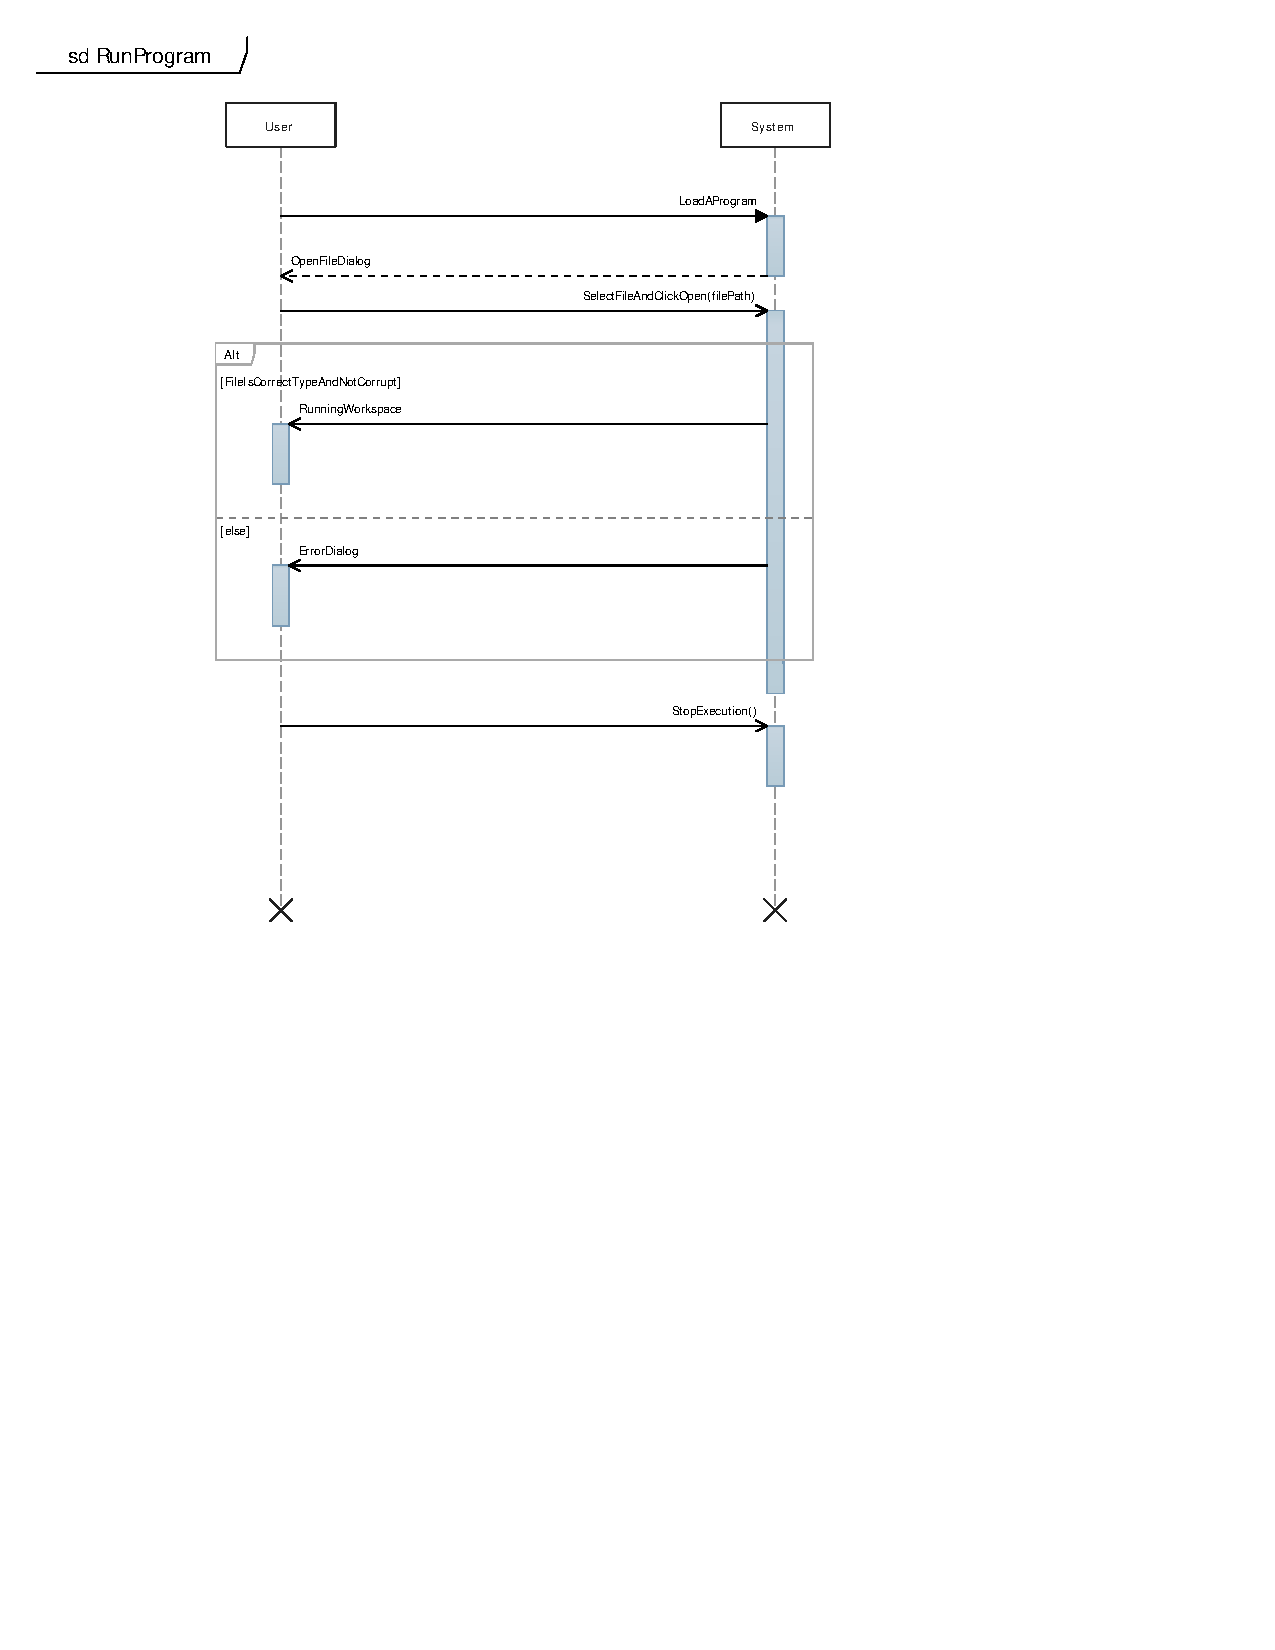
\includegraphics[scale=1]{./pdfs/MS4Models/LoadProgram.pdf}
\end{center}

\section{Sequence Diagrams}

\begin{center}
        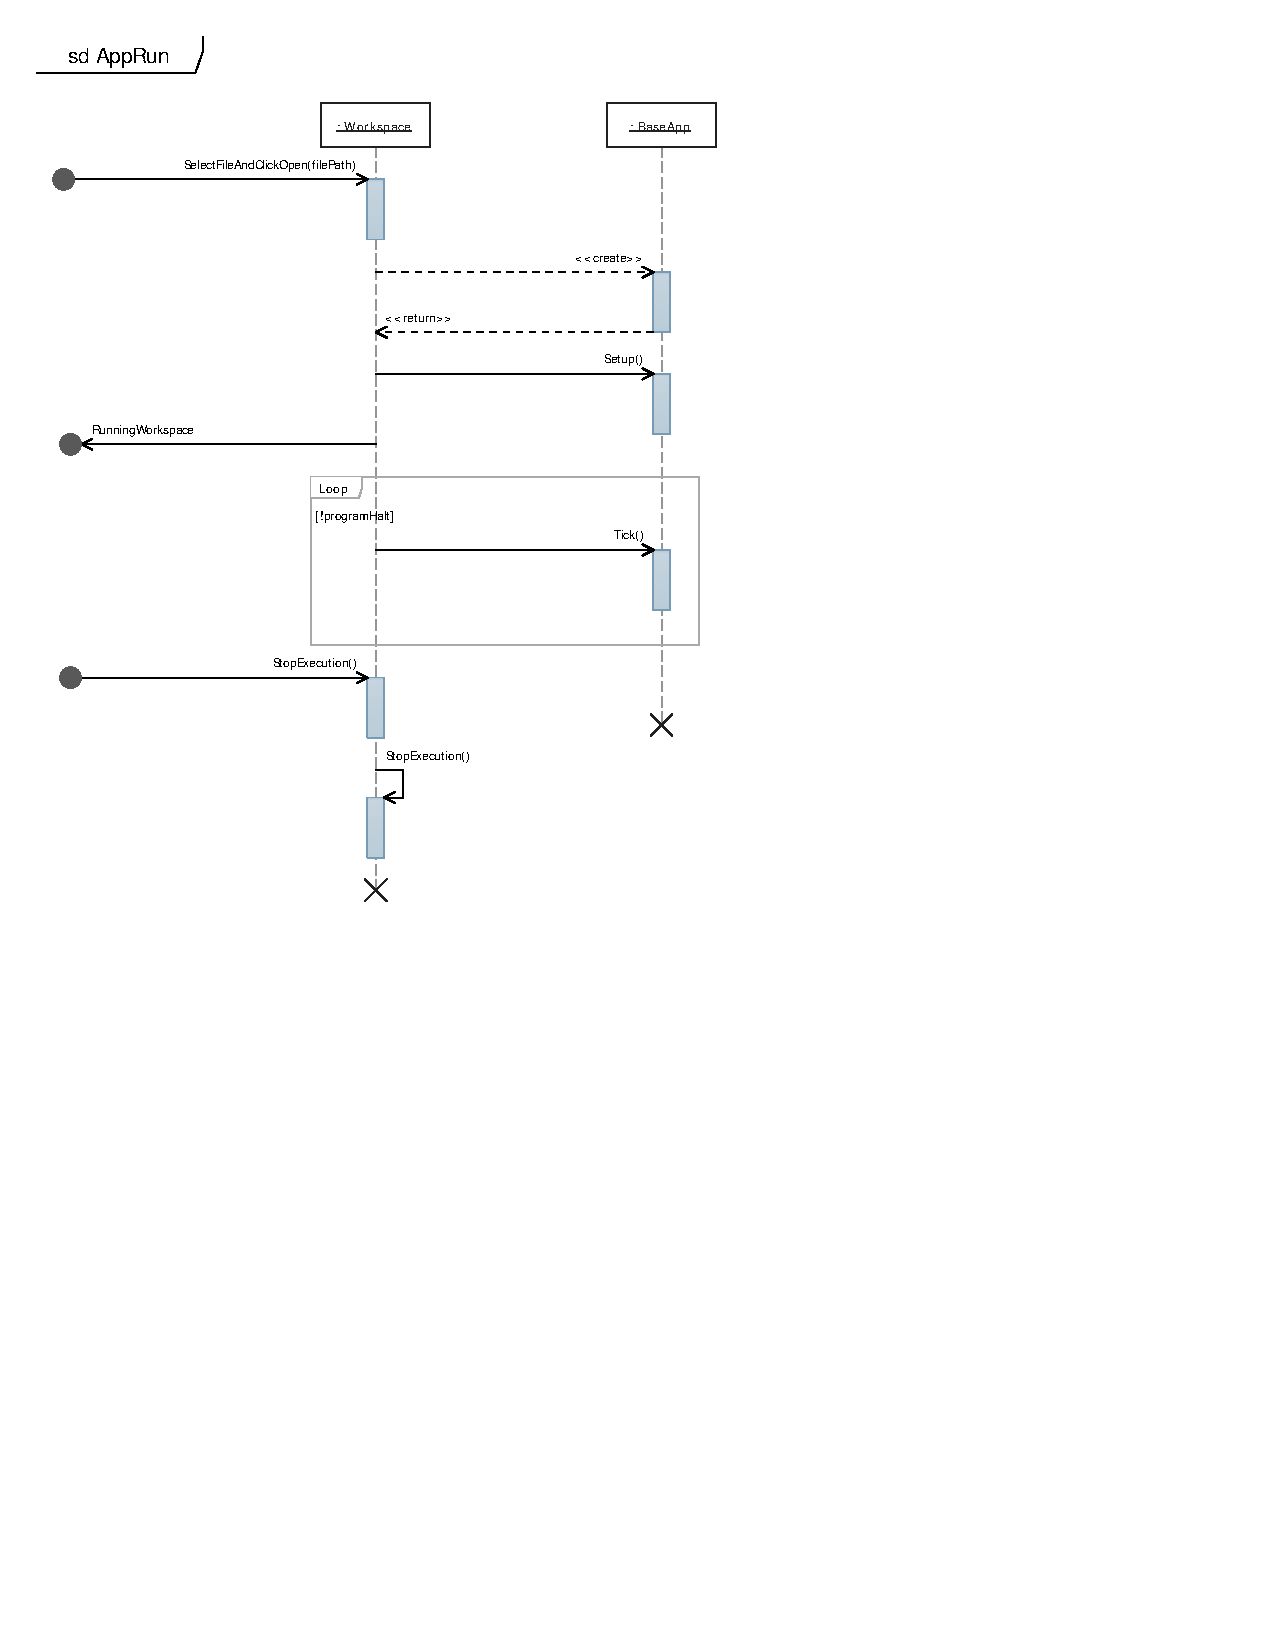
\includegraphics[scale=1]{./pdfs/MS4Models/ReflexGame.pdf}
\end{center}
The \textit{Setup()} operation is necessary in addition to a constructor because this is the way in which initialization of an application is handled per Sifteo's API. No changes were made to this sequence diagram because it is consistent with the way in which the system behaves during this operation.

\begin{center}
        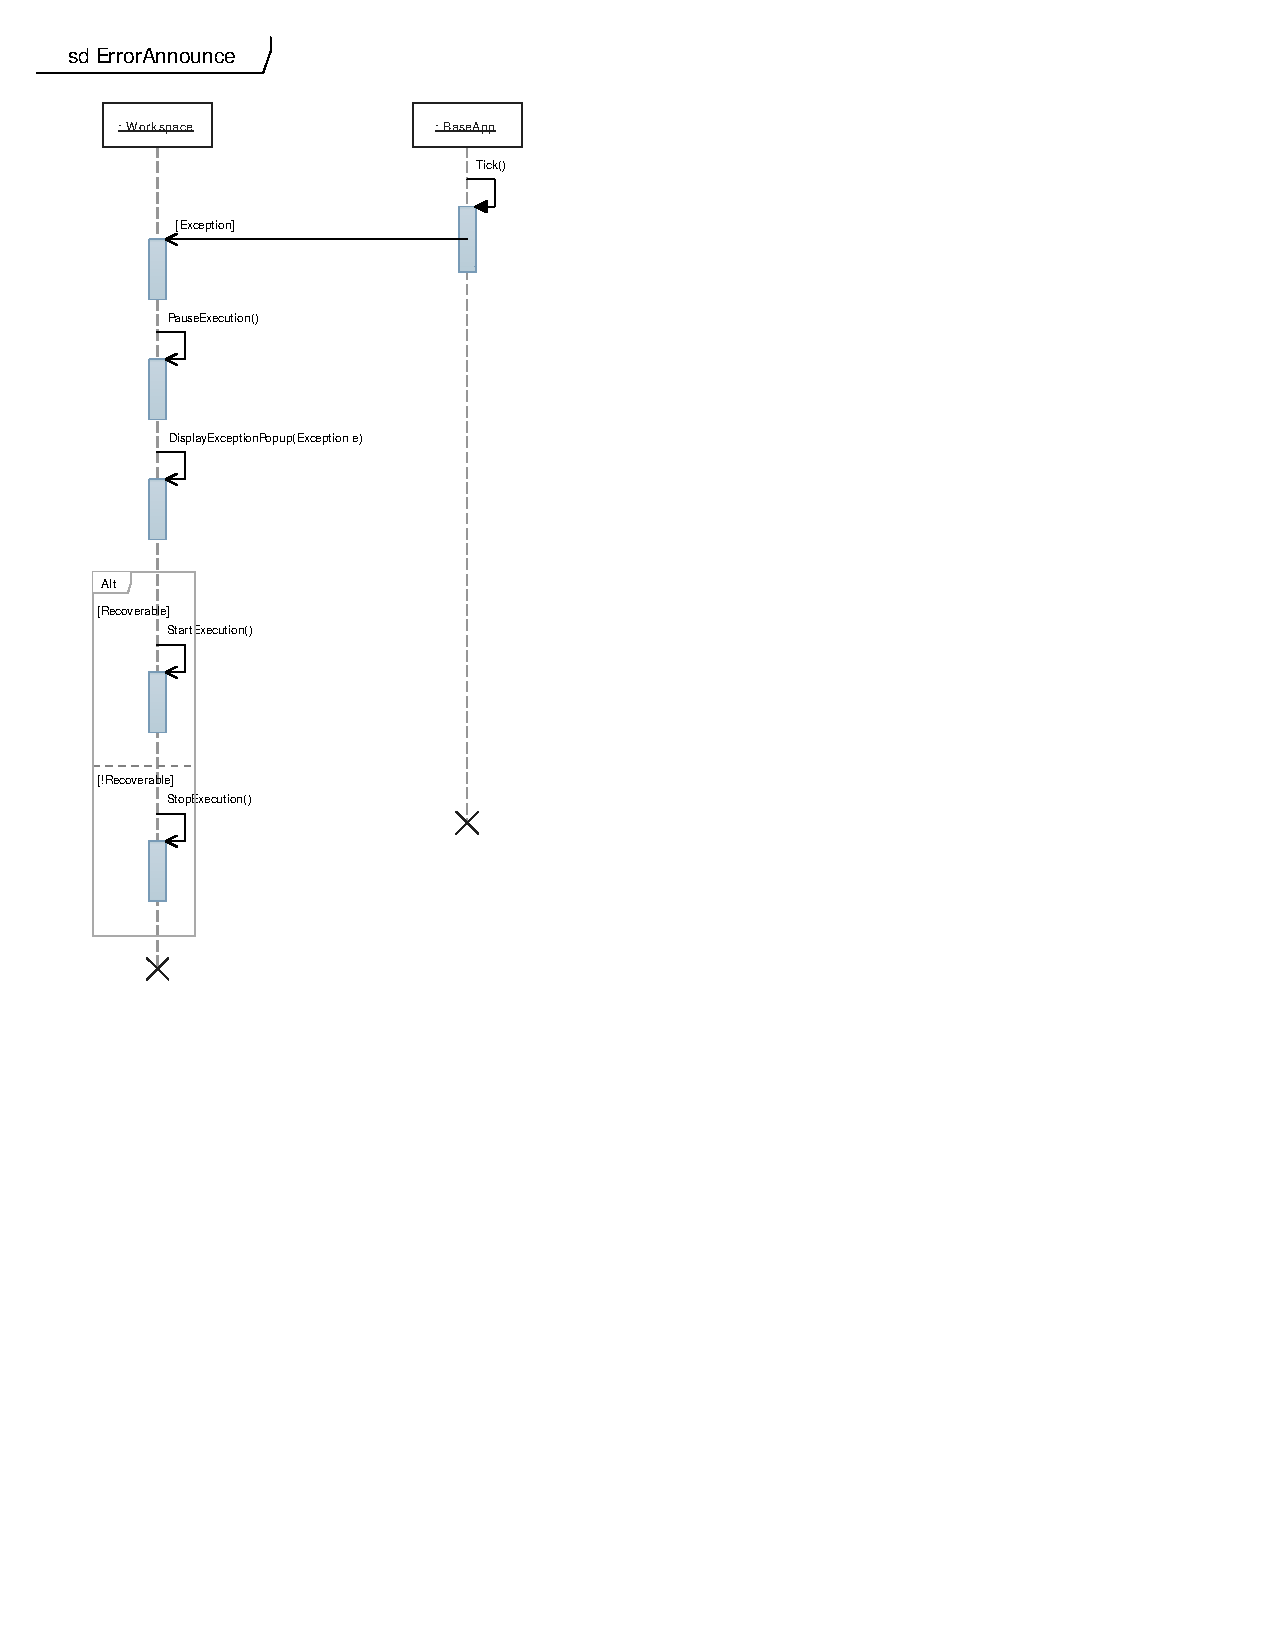
\includegraphics[scale=1]{./pdfs/MS4Models/ErrorAnnounce.pdf}
\end{center}
The \textit{Tick()} operation was unintentionally omitted from the original diagram, and it has been added for clarity to indicate that the action is taking place during an actively running application.

\section{Design Class Diagram}
Any external relationships our shown beneath the class name to emphasize interaction with classes we did not create. For instance, each \textit{Cube} is implemented as a \textit{UserControl} object.
\\\\
Additionally, every entity in our diagram is being implemented in our own original code, though many classes are inspired by the Sifteo API which we have to mirror. Those entities which do mirror the objects in the Sifteo domain will be separated into a distinct package to clarify the divide between those objects which carry out the emulation and those which the user primarily manipulates in their original applications.

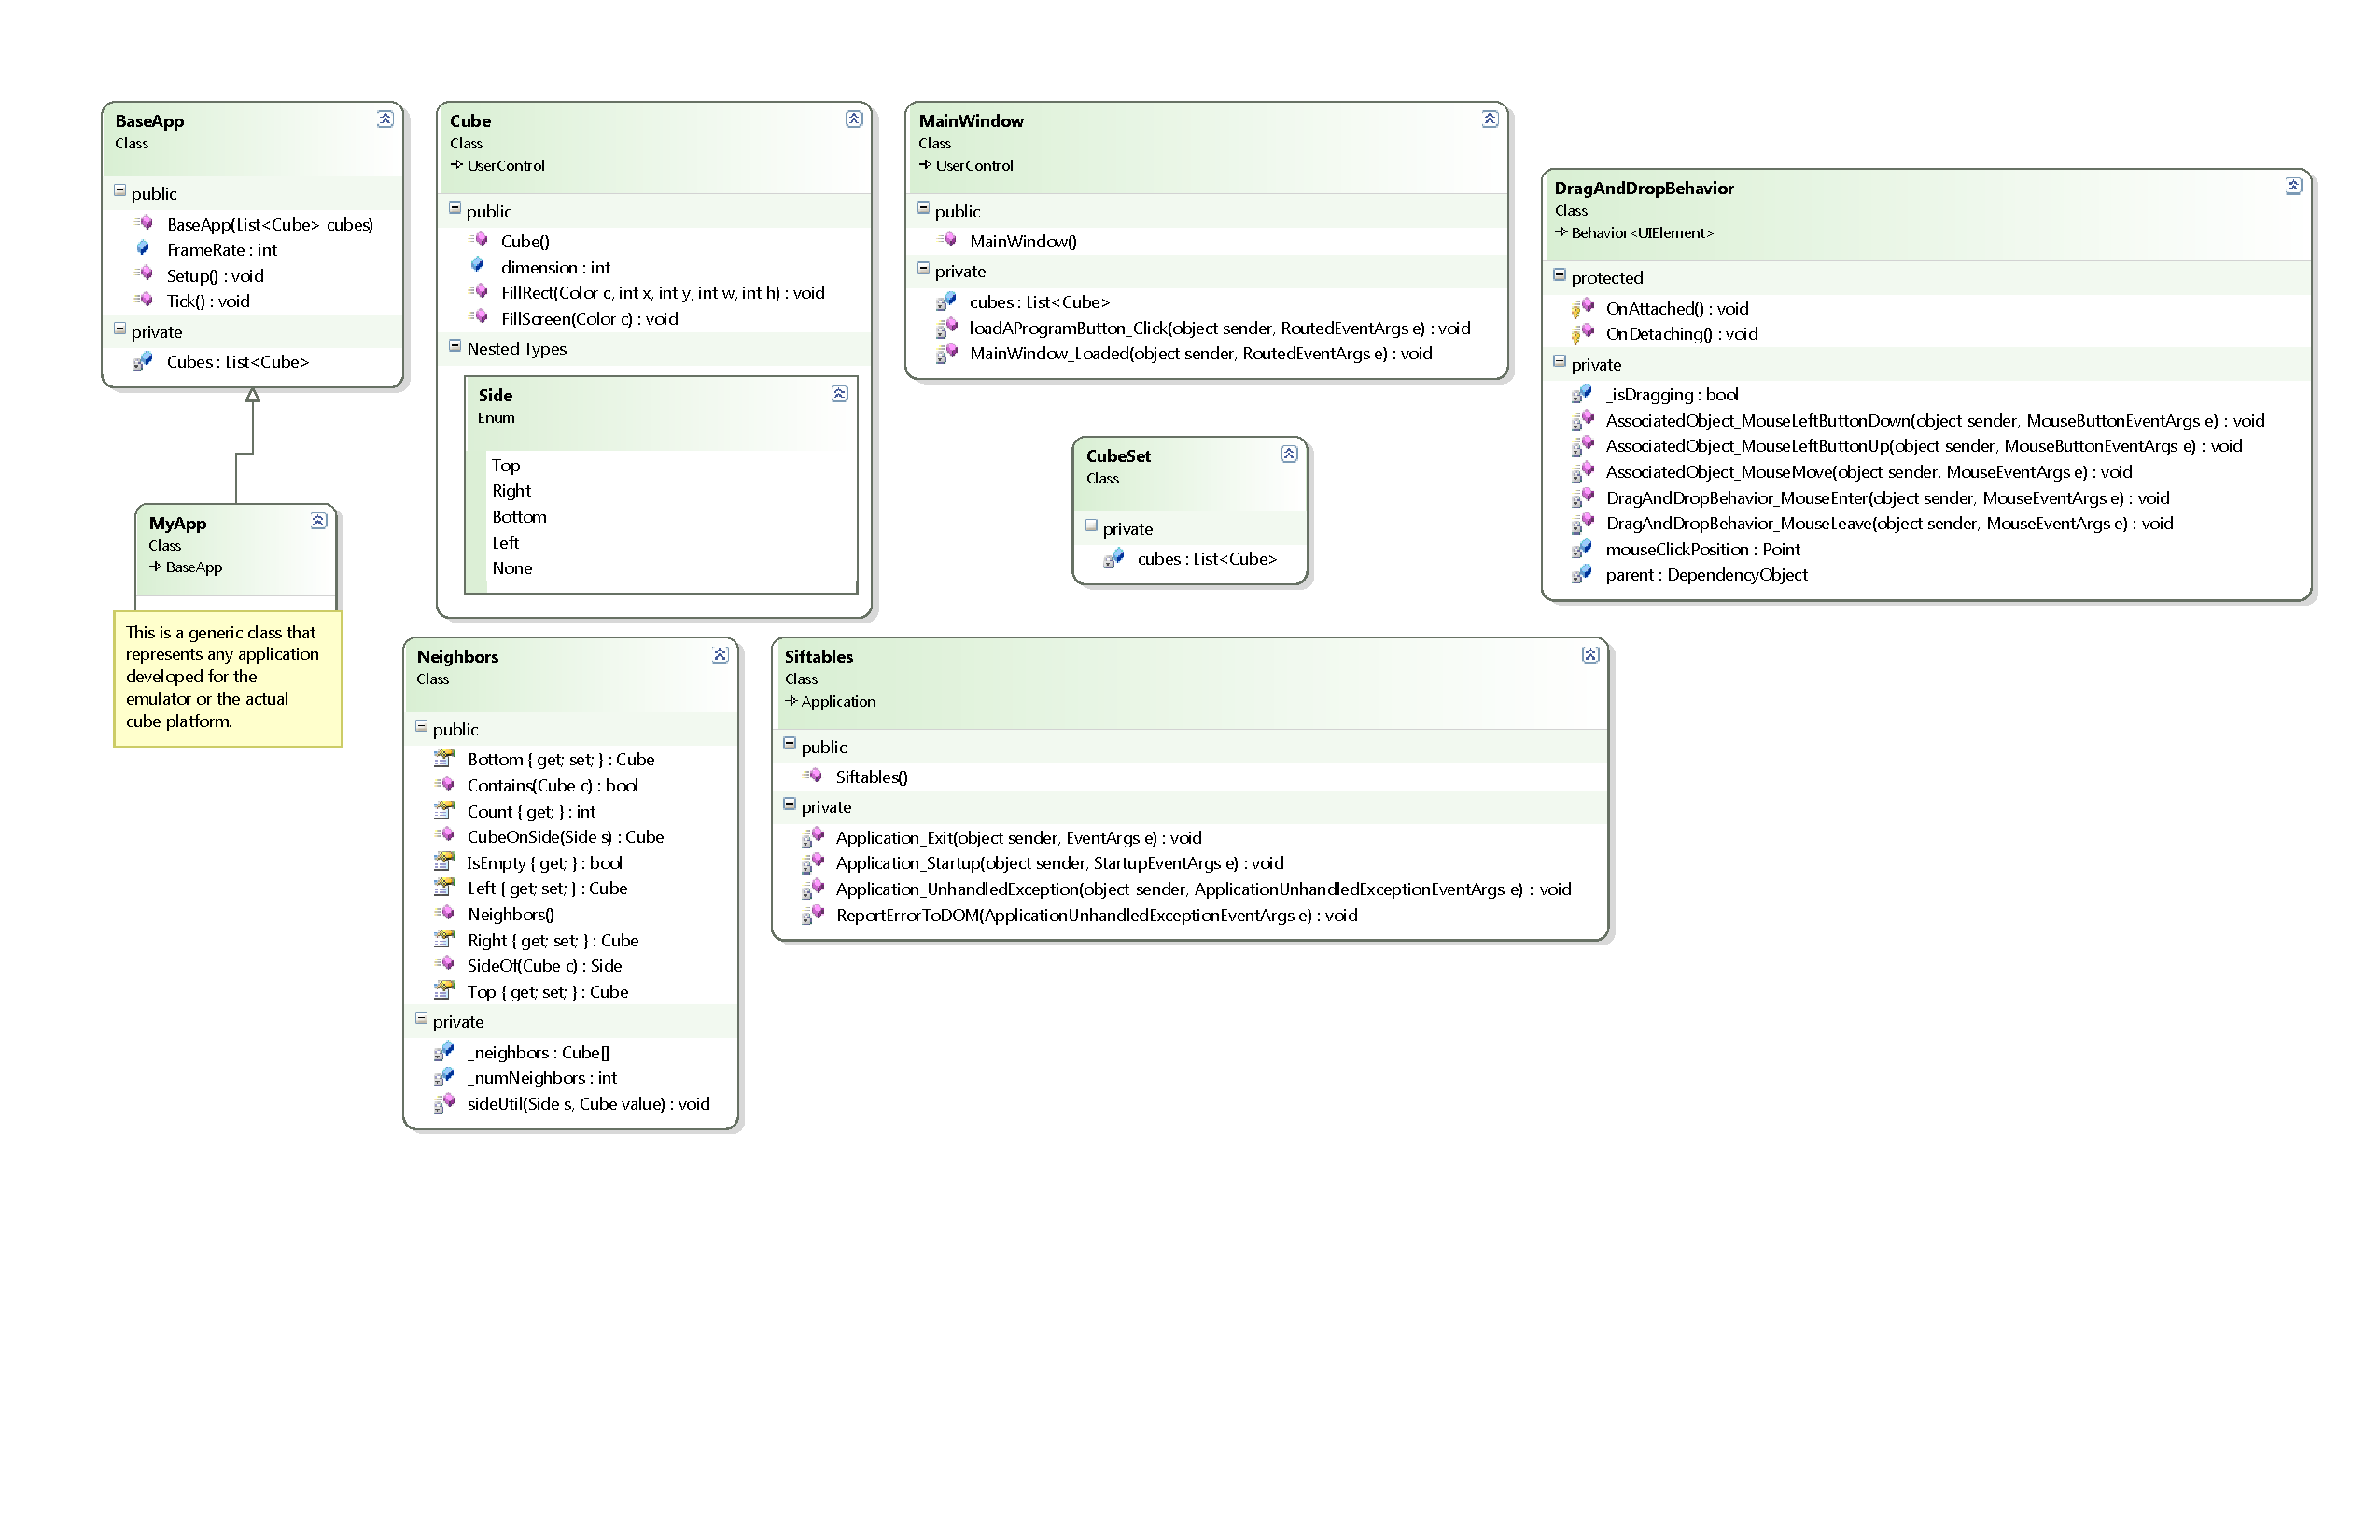
\includepdf{./pdfs/MS4Models/ClassDiagram.pdf}

\textbf{Note}: Because the class diagram was generated by Visual Studio, no associations were created (for instance, between the entity \textit{Cube} which is associated with a unique \textit{Neighbors} entity). We feel no clarity was lost by ommitting these associations.

\section{Applications of the GRASP Principles}

\subsection{Creator}
\textit{MainWindow} creates each of the cubes because it has the information (location in the space) necessary to construct them. Also, the \textit{Siftables} entity is responsible for creating \textit{MainWindow} because it acts as the starting point for the emulator.

\subsection{Information Expert}
Because each \textit{Cube} object is the sole owner of the information (in this case, a collection of graphical objects) which are contained on its screen, it is responsible for conveying this in the workspace onto the graphical representation of its screen.

\subsection{Controller}
There is no concrete example of a controller in our design, but \textit{BaseApp} acts like a use case controller because it is in charge of handling interactions between domain-level objects and the user interface (on the \textit{Cube} screens). Though we are not sure which entity will have this responsibility, there will also be a controller (or dispatcher) to begin the emulation of an application and handle the calls to \textit{Tick()} which will subsequently cause changes to the interface.

\subsection{Low Coupling}
\textit{BaseApp} only connects to the UI layer simply through the \textit{Cube} entities because it is responsible for controlling events related to the cubes and must be responsible for carrying out the steps specified in each application. This reduces coupling between the two logical layers and allows the domain layer to be implemented more independently from the interface layer.

\subsection{Pure Fabrication}
The \textit{Neighbors} entity does not exist in the physical domain, but it is useful in the implementation to separate the responsibility of keeping track of a cube's neighbors and their interactions from the graphical representation of the cube. The \textit{CubeSet} class represents the set of cubes which exist in the current workspace, which is maintained as a separate entity to allow events to be defined on the entire set of cubes. For instance, an event can be triggered when a cube is added or removed from the set, which could not easily be handled if a set of cubes was implemented simply as a data structure.

\subsection{High Cohesion}
The \textit{Cube}, \textit{Neighbors}, and \textit{CubeSet} class all emphasize high cohesion by abstracting out specific, distinct responsibilities to separate entities. The \textit{Cube} acts primarily as a graphical interface to the cube objects, while \textit{Neighbors} has the responsibility of maintaining neihborhood relationships between \textit{Cube} objects. The \textit{CubeSet} responsibilities are mentioned above.

\subsection{Protected Variations}
While our system does not directly intereact with third-party interfaces, and therefore does not directly use the Protected Variations pattern, the project as a whole is itself a Protected Varation that implements the Sifteo API. An overriding goal of our design going forward will be to remain fully compatible with that API so that applications written for the actual Sifteo Cube platform can also be run on our emulator.
\\\\
\textbf{Note}: Because our system does not interact with third-party interfaces, there are not clear examples of the \textbf{Indirection} pattern.
        
\end{document}
